\subsection{22 августа. Д.р. Джалпаккол}
\textit{Метеоусловия: утром, днём ясно, вечером~--- переменная облачность, тепло. Ночью сильная гроза.}

\begin{figure}[h!]
	\centering
	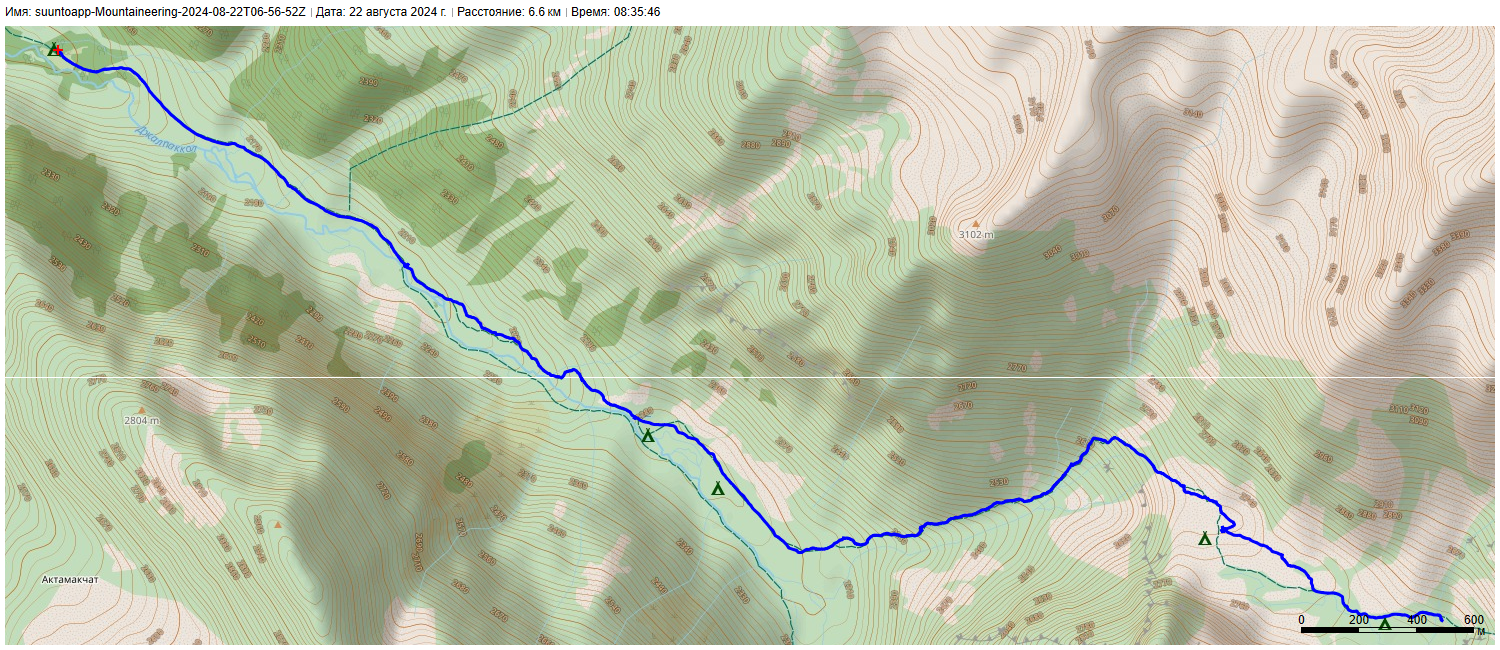
\includegraphics[angle=0, width=0.7\linewidth]{../pics/mini_maps/22}
	\label{fig:mini_22}
\end{figure}


\begin{figure}[h!]
	\centering
	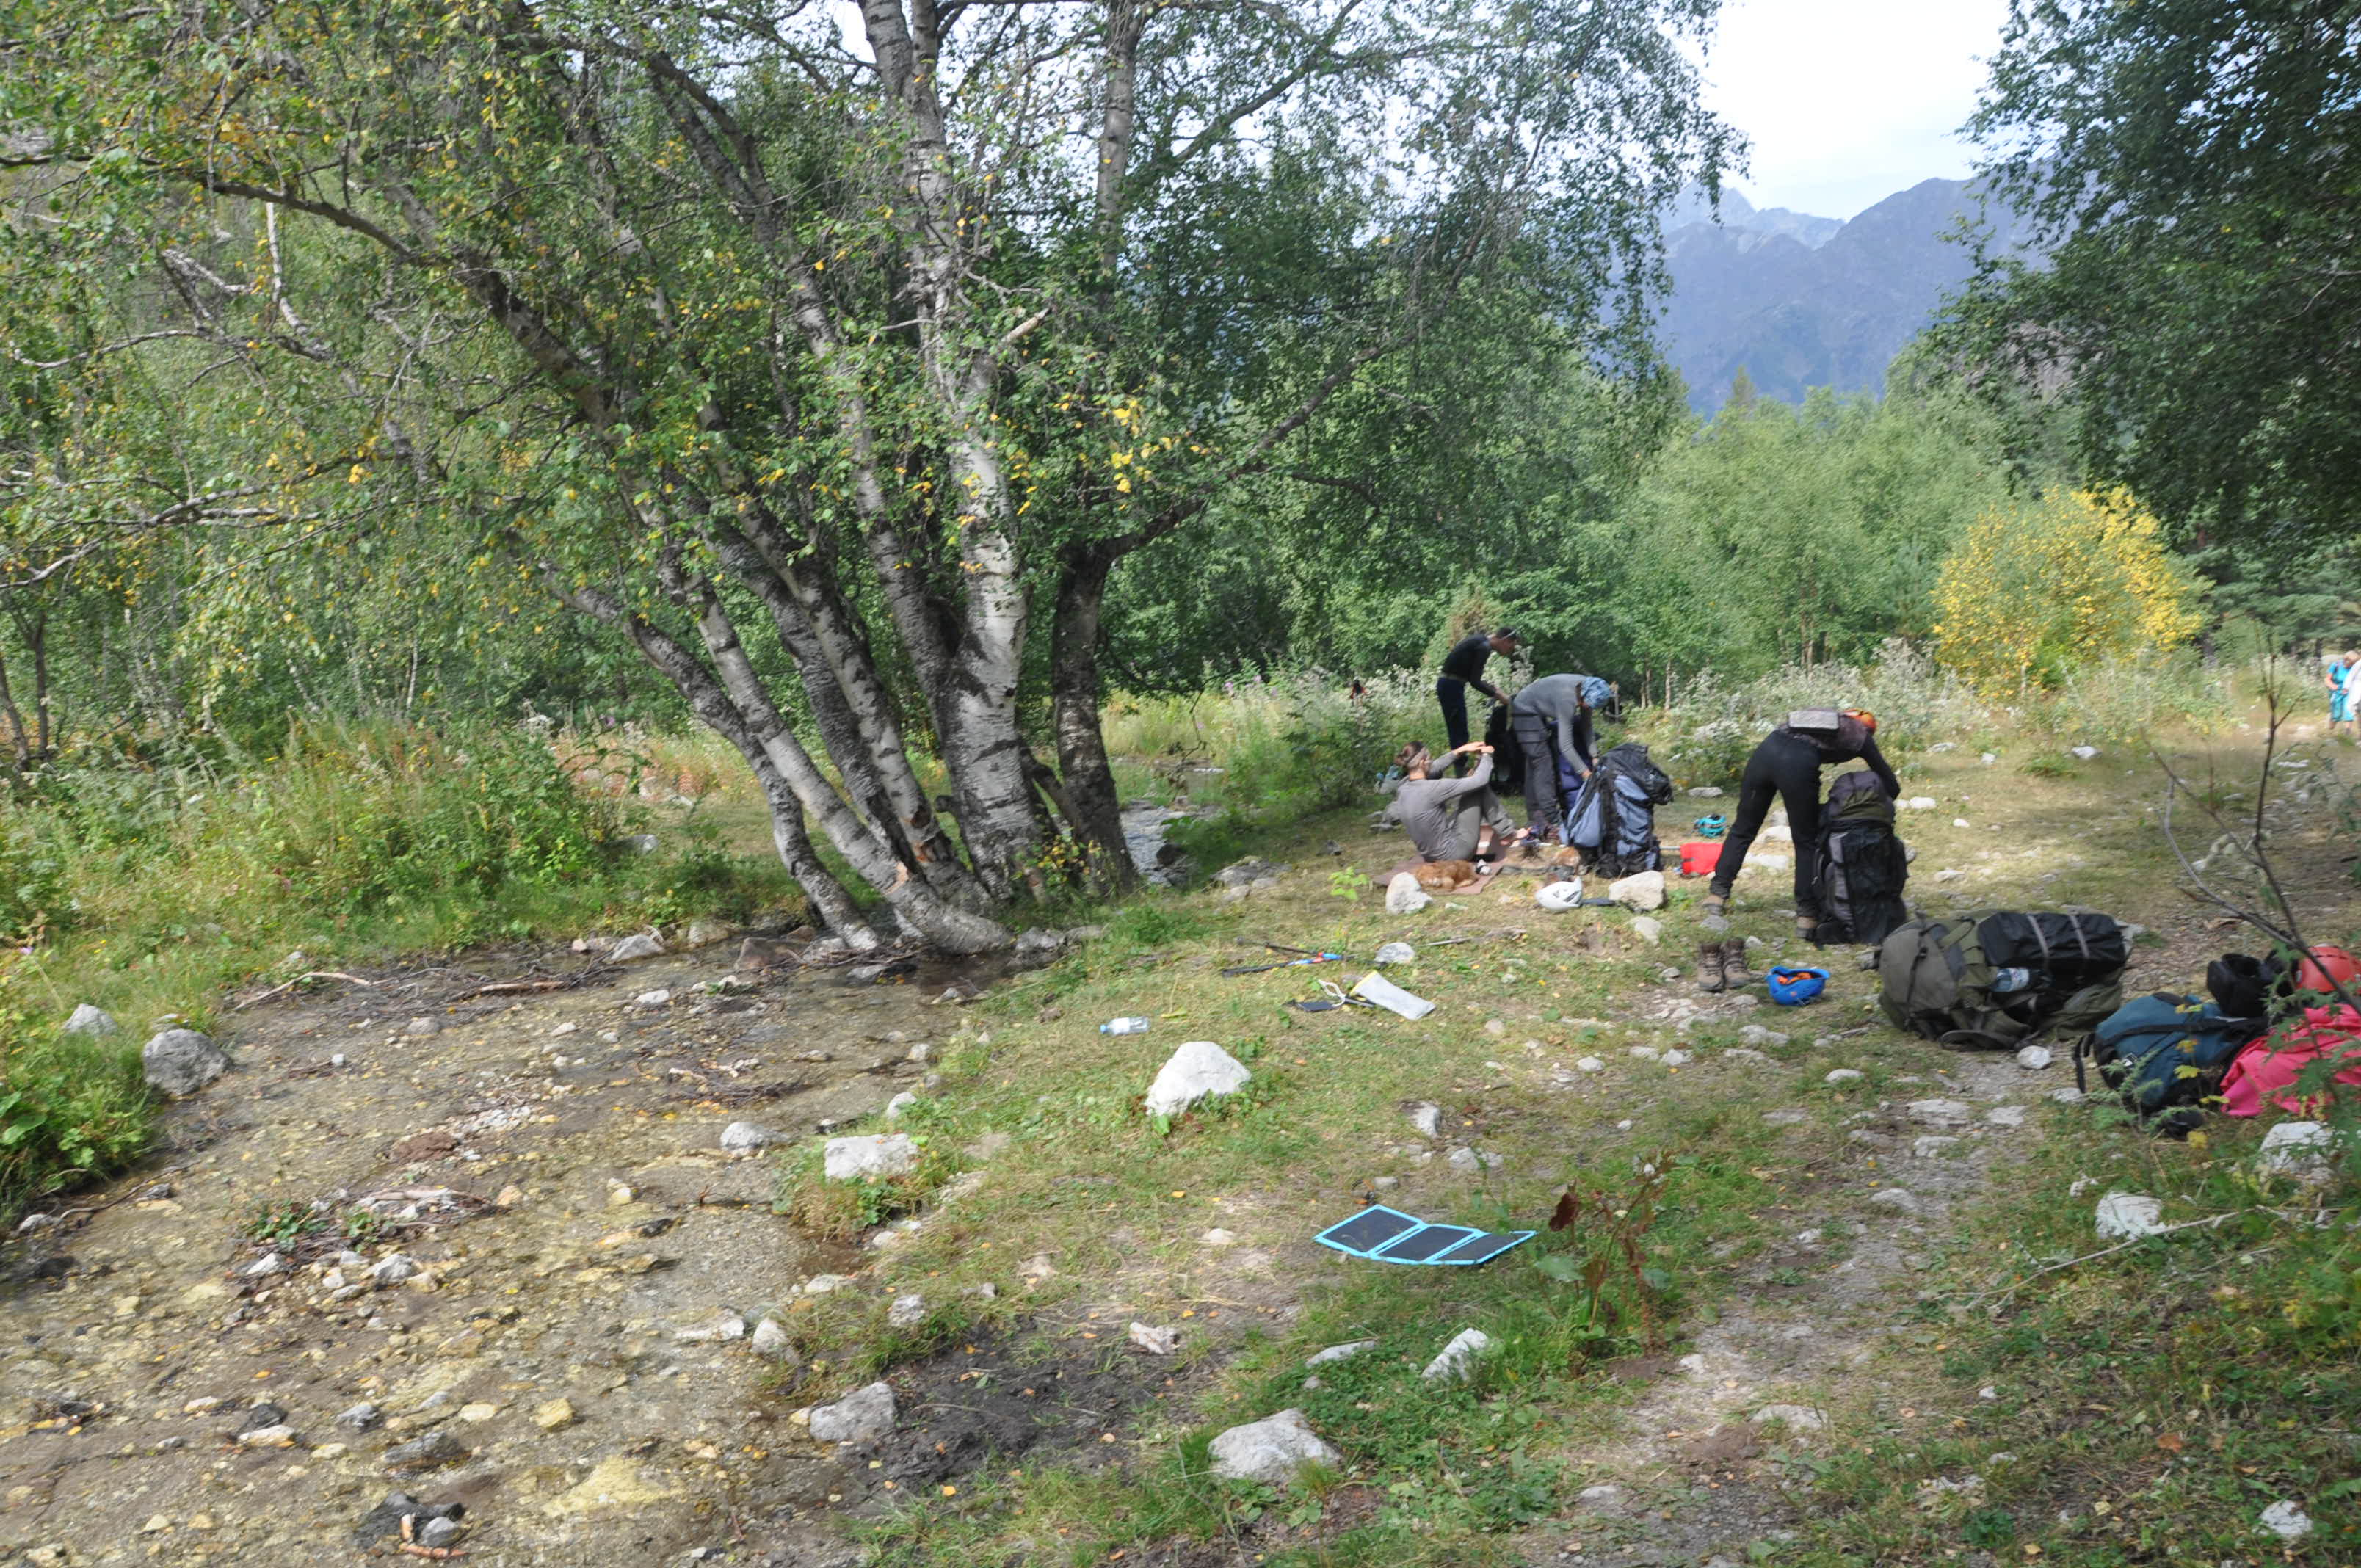
\includegraphics[width=0.7\linewidth]{../pics/DSC_1181}
	\caption{Место ночёвки 21-22.08. Утренние сборы}
	\label{fig:DSC_1181}
\end{figure}


Из-за позднего завершения ходового дня накануне устраиваем подъём достаточно поздно, в 08:00, и выходим в 10:00 (рис. \ref{fig:DSC_1181}). Движемся по правому берегу р. Джалпаккол, не переходя на левый берег у коша N 43.296700\degree,~E 42.046662\degree. Тропа хорошо набита, место часто посещаемо: обогнали группу пенсионеров, поднимавшихся от т/б <<Глобус>> к водопадам д.р. Кичкинекол Джалпаккольский. Любуемся бесконечными полянами крокусов (рис. \ref{fig:IMG_20240822_101505}).

\begin{figure}[h!]
	\centering
	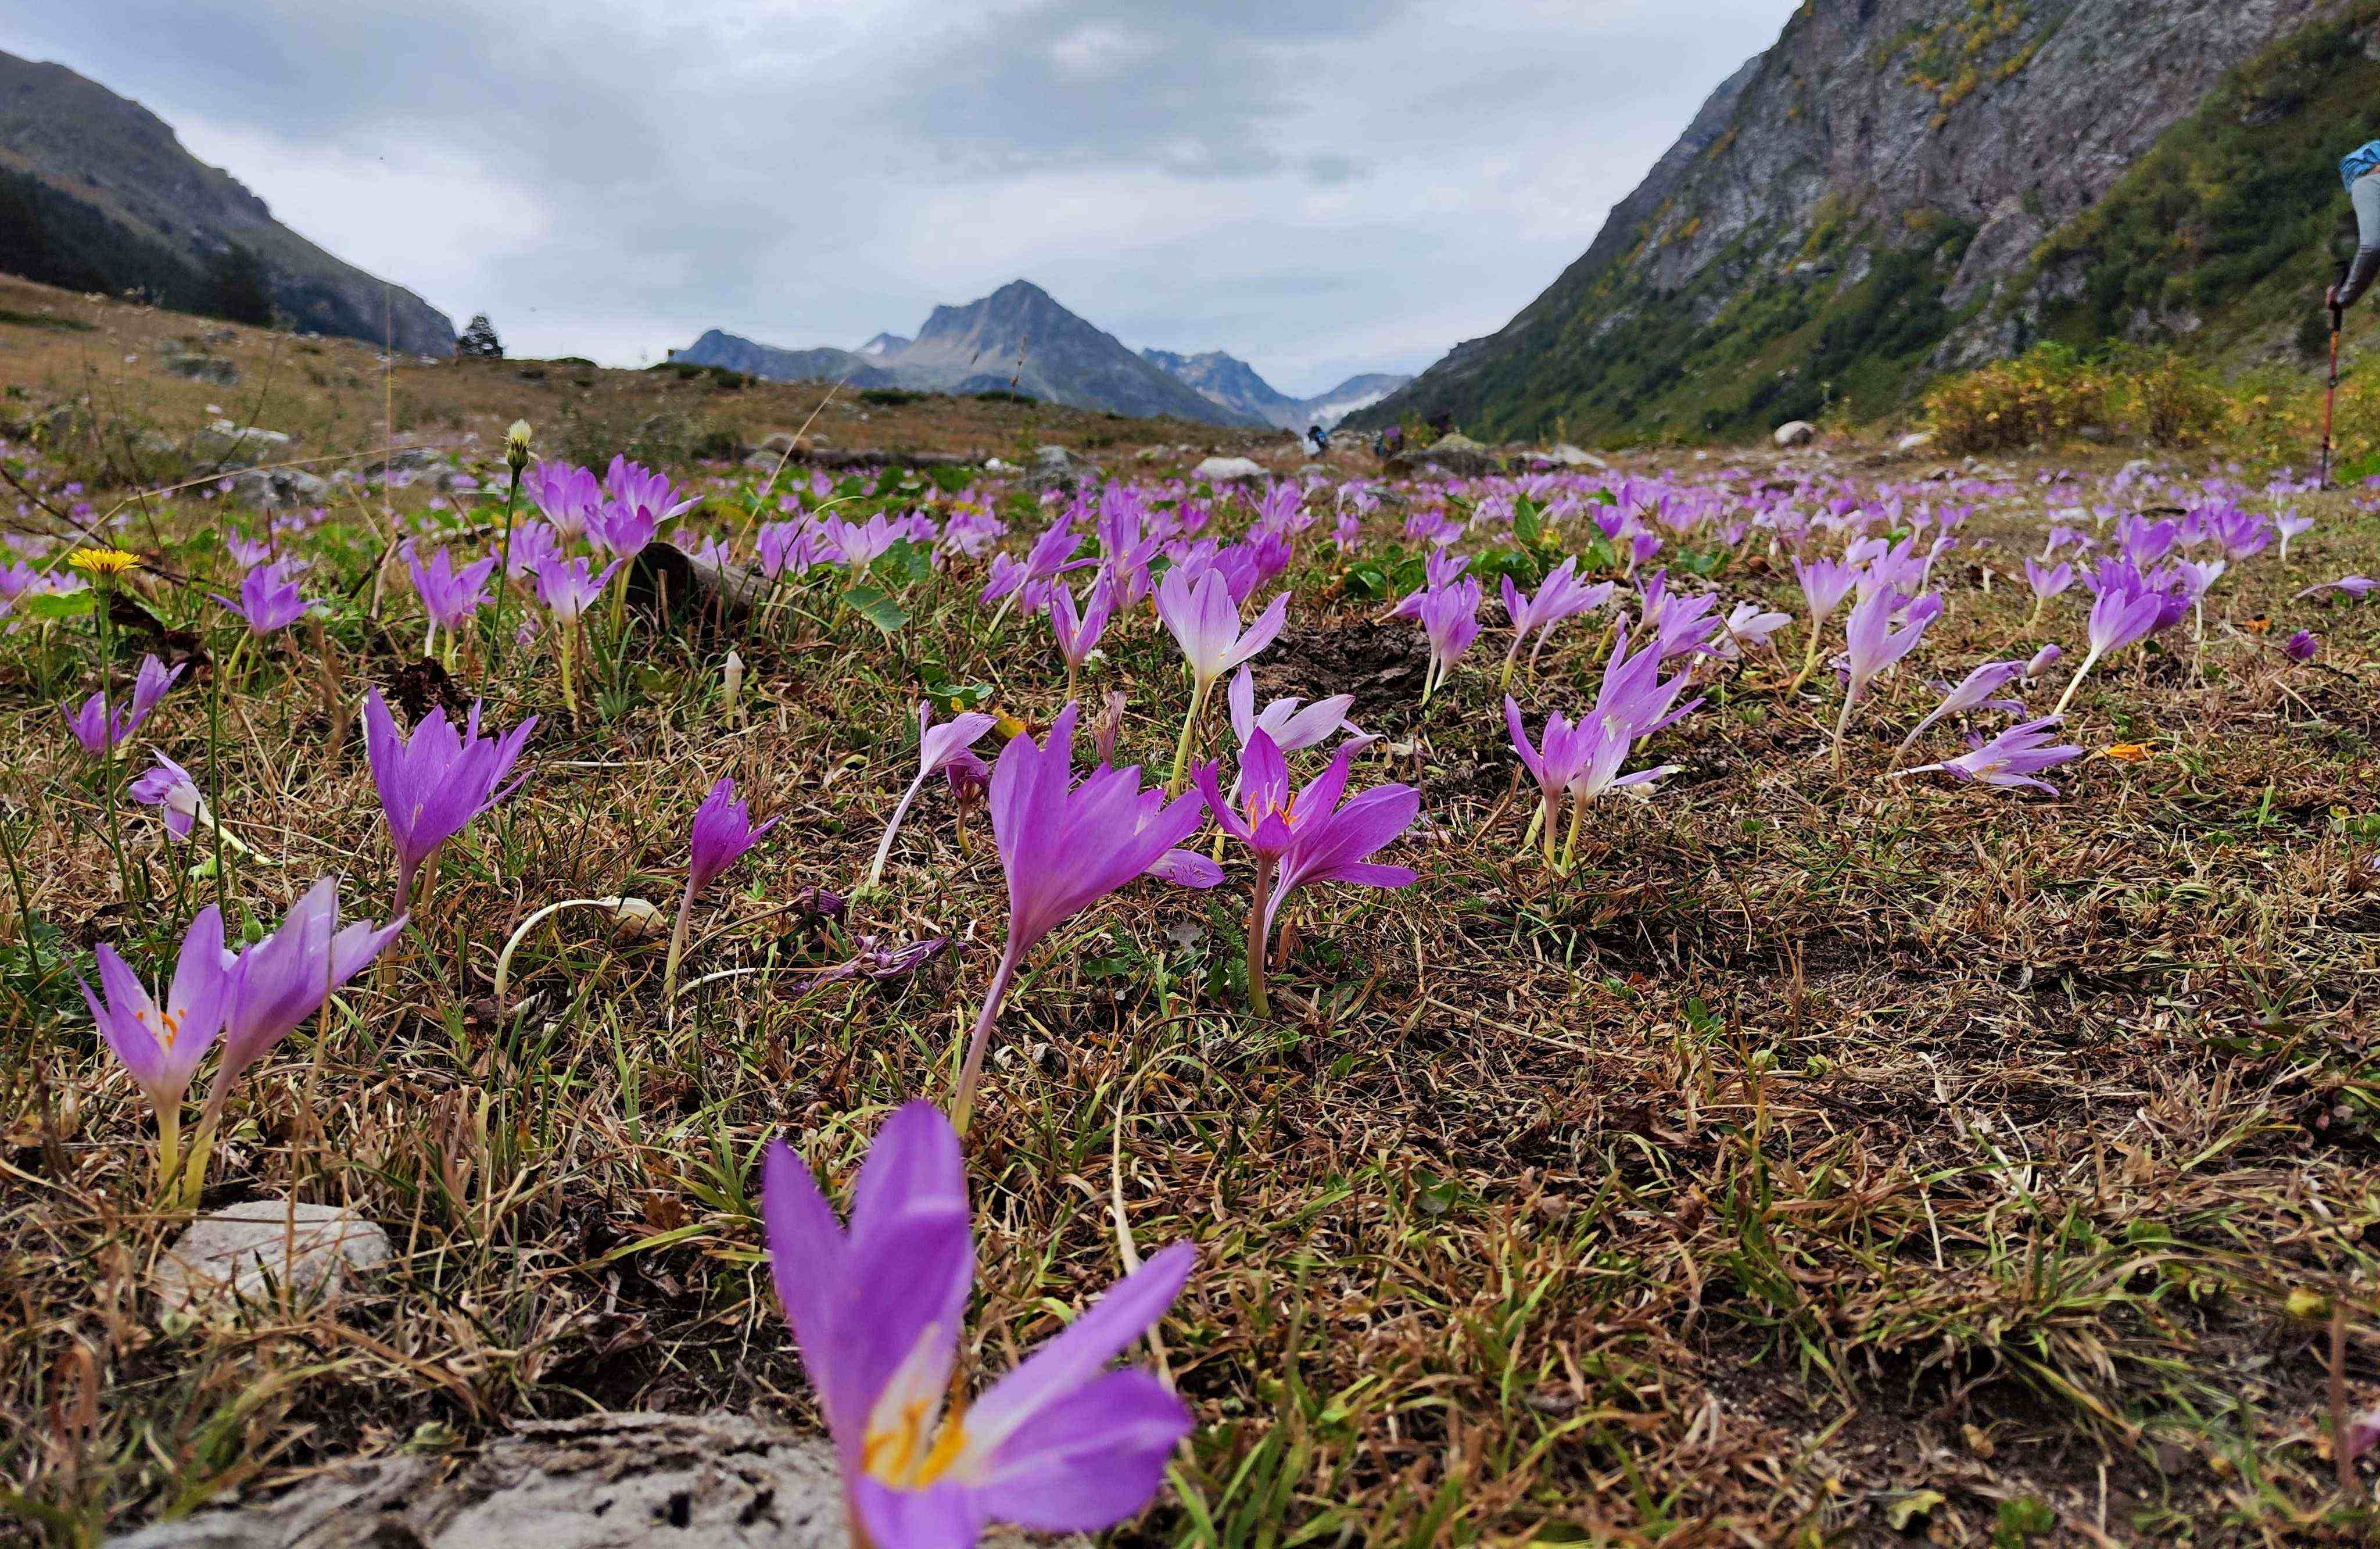
\includegraphics[width=0.7\linewidth]{../pics/IMG_20240822_101505}
	\caption{Крокусы в д.р. Джалпаккол}
	\label{fig:IMG_20240822_101505}
\end{figure}

В 11:45 дошли до развилки: направо пхд~--- верховья д.р. Джалпаккол, налево~--- д.р. Кичкинекол Джалпаккольский. Место живописное: плоская долина Джалппаккола (откуда и карачаевское название) как на ладони, в ущелье Кичкинекола шумит река, впереди открывается вид на хребет Куршо. Останавливаемся на фотопривал, фотографируемся (рис. \ref{fig:DJI_0830}).

\begin{figure}[h!]
	\centering
	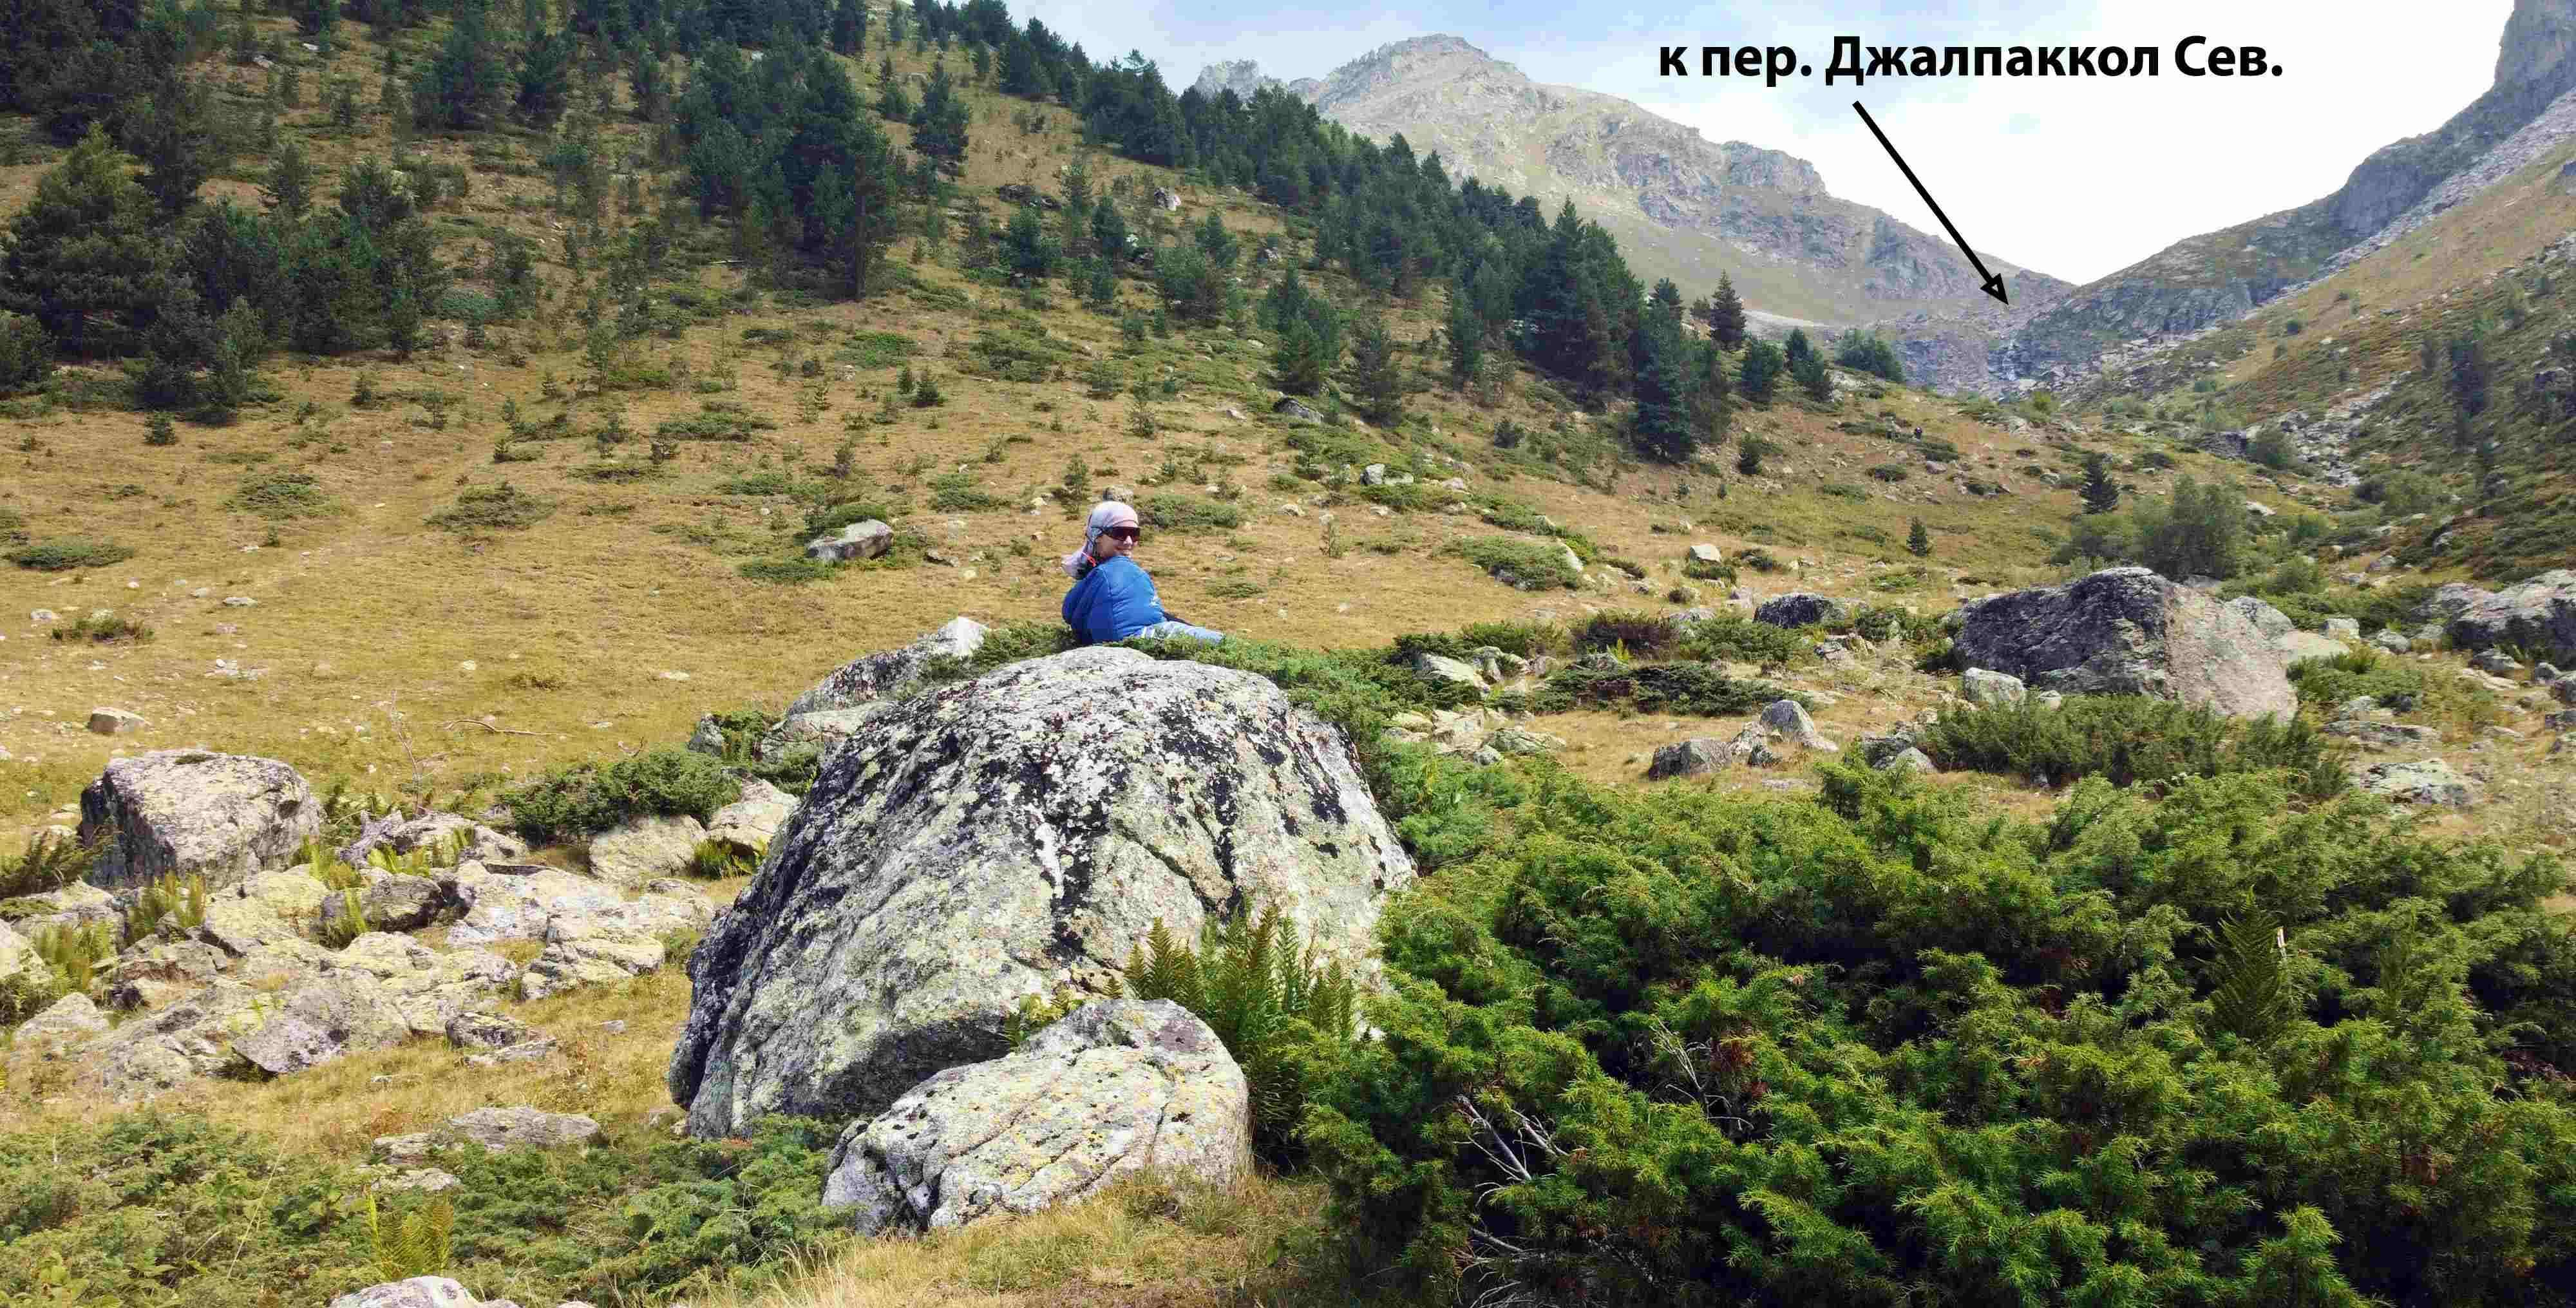
\includegraphics[width=0.7\linewidth]{../pics/DJI_0830}
	\caption{На фотопривале}
	\label{fig:DJI_0830}
\end{figure}

Далее движемся по хорошо набитой и промаркированной тропе по ущелью Кичкинекола Джалпаккольского. Обходим бараньи лбы и водопады слева пхд (рис. \ref{fig:DJI_0835}).


\begin{figure}[h!]
	\centering
	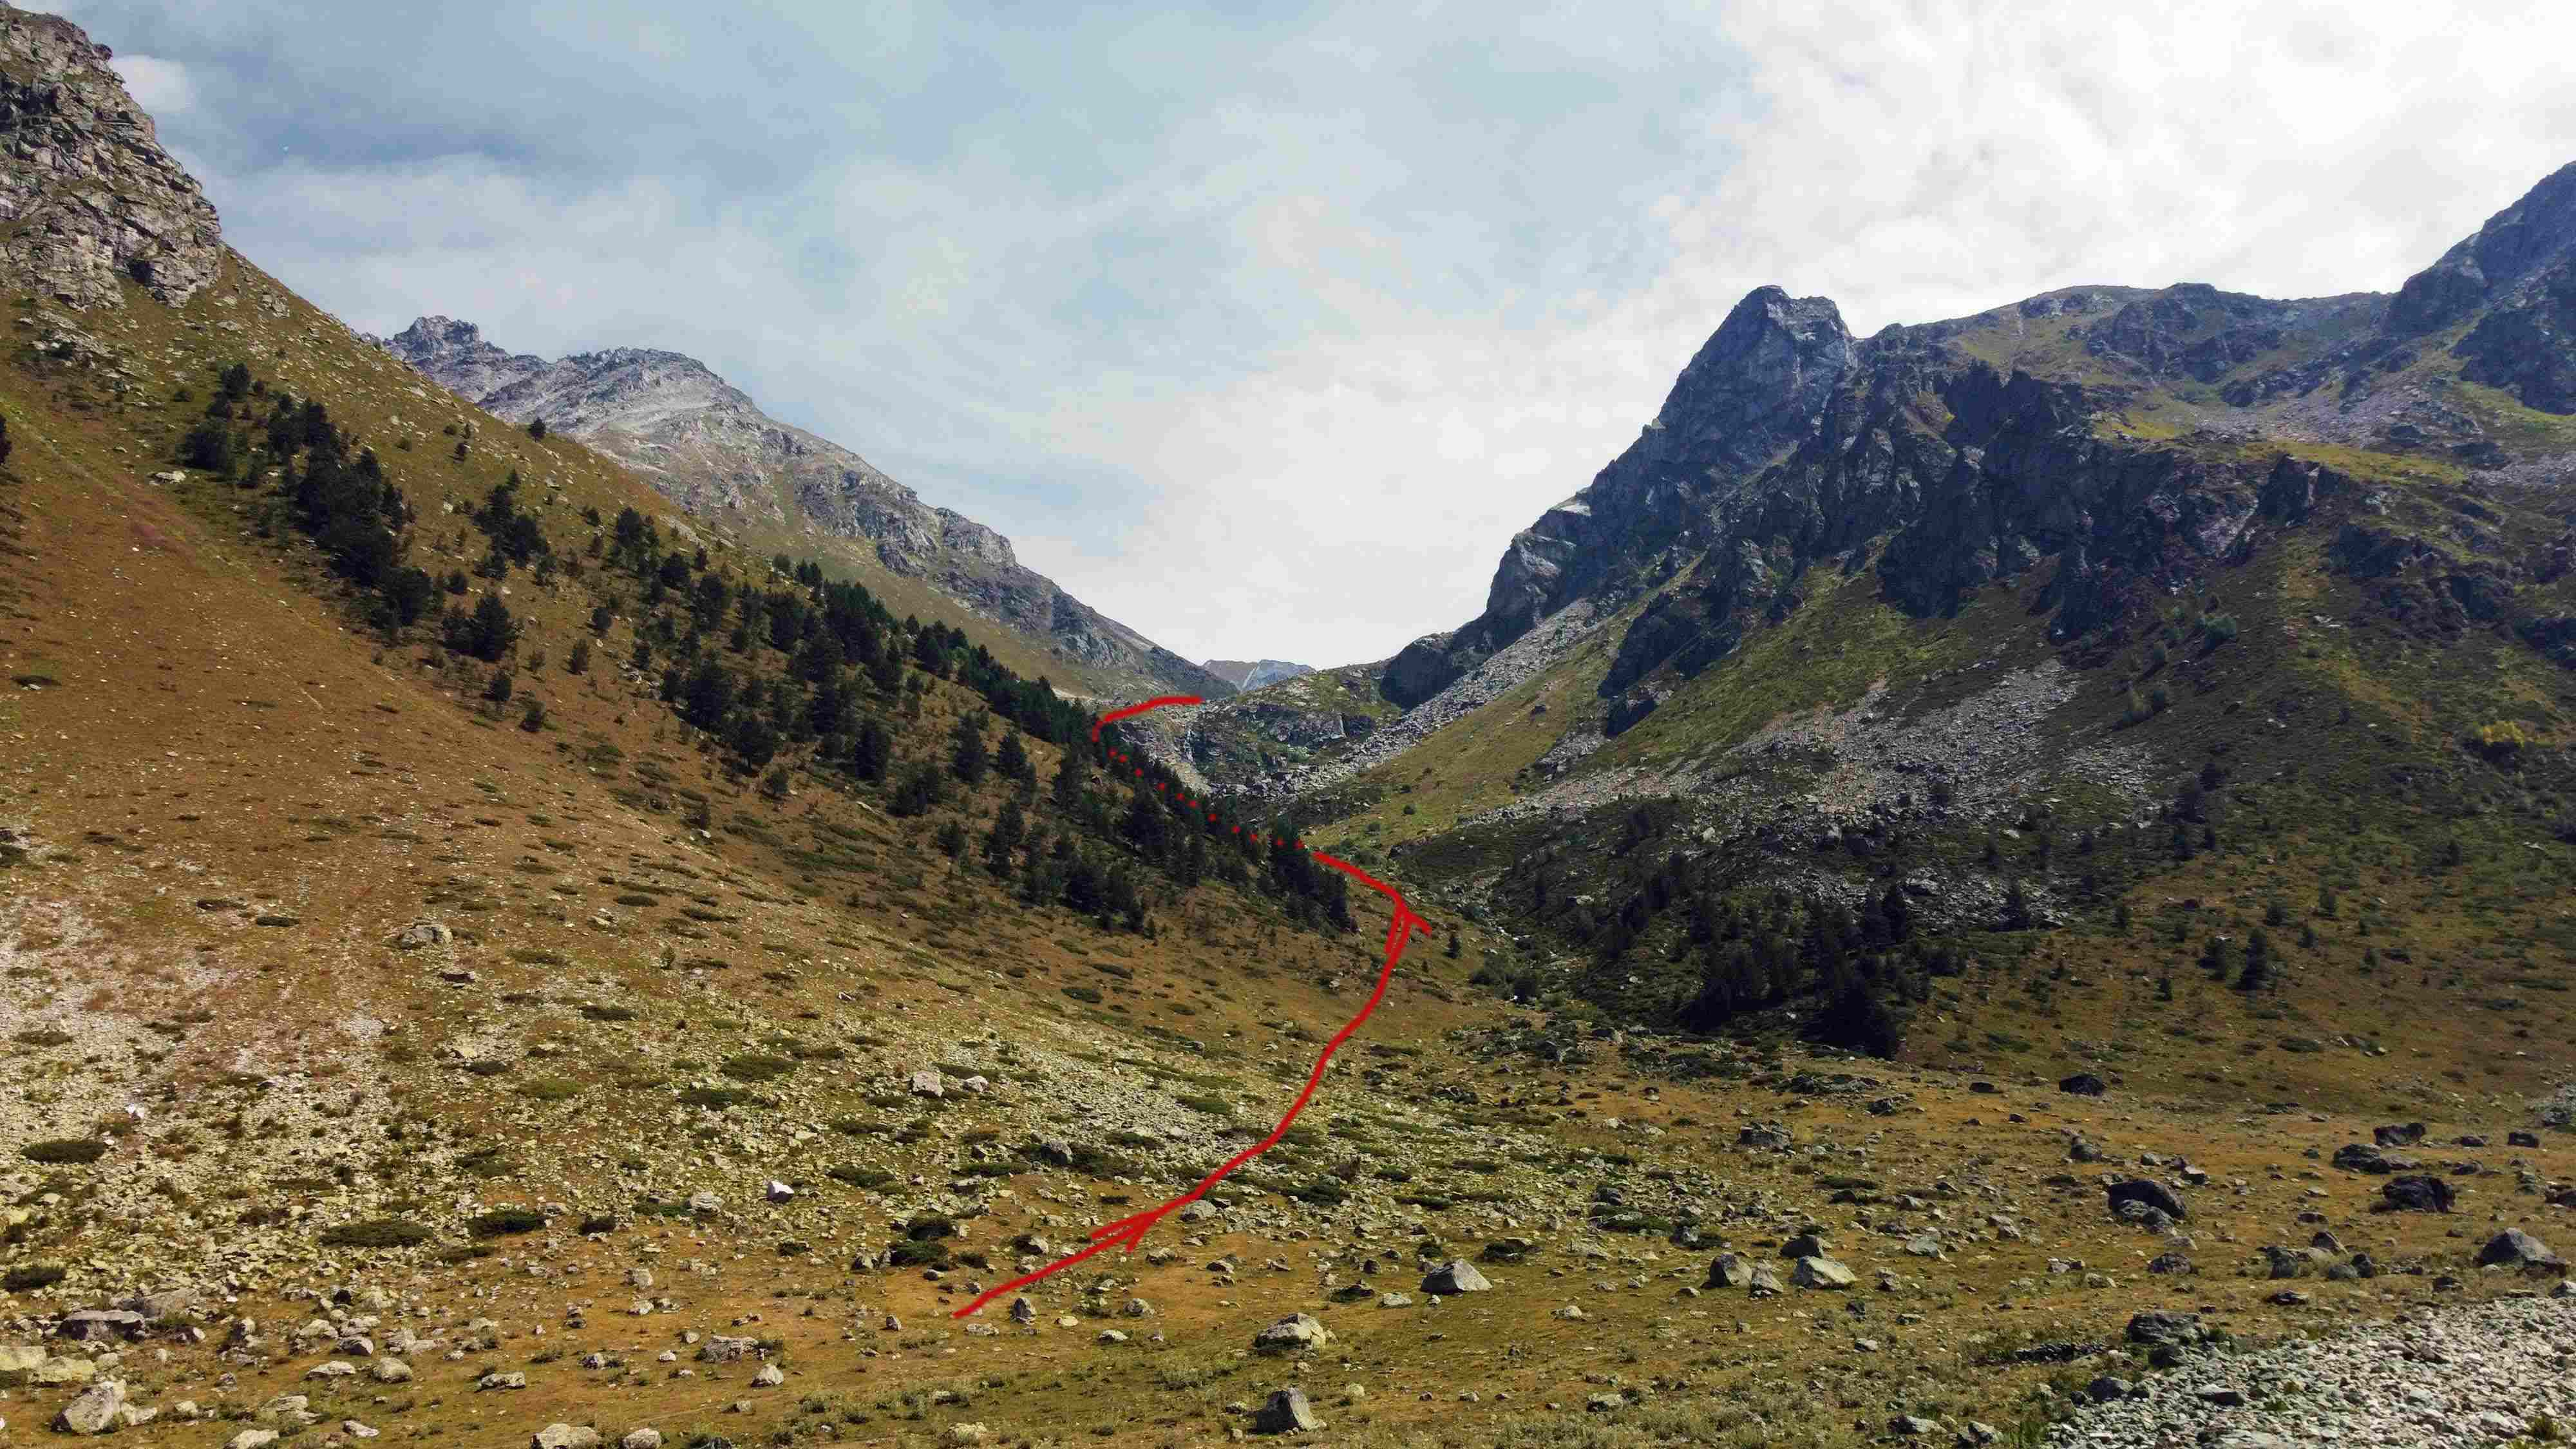
\includegraphics[width=0.7\linewidth]{../pics/DJI_0835}
	\caption{Маршрут подъёма в д.р. Кичкинекол Джалпаккольский из д.р. Джалпаккол}
	\label{fig:DJI_0835}
\end{figure}

За водопадами на древней морене нас обгоняет группа коммерческих туристов. Инструктор группы удивляется тому, что мы в рамках похода 1 к.с. идём перевал Джалпаккол Северный.

Поднявшись на моренный вал, в 15:45 устраиваем обед на оборудованной стоянке (N~43.288482\degree, E~42.081736\degree). Во время обеда устраиваем разведку, по итогам которой решаем ночевать за следующей моренной ступенью на верхних зелёных стоянках (N~43.285565\degree, E~42.091178\degree, рис. \ref{fig:DSC_0018}), куда приходим в 18:30. Глубокой ночью (примерно с 01:00 по 03:00) разразилась сильная гроза с частыми молниями и сильным ливнем.

\begin{figure}[h!]
	\centering
	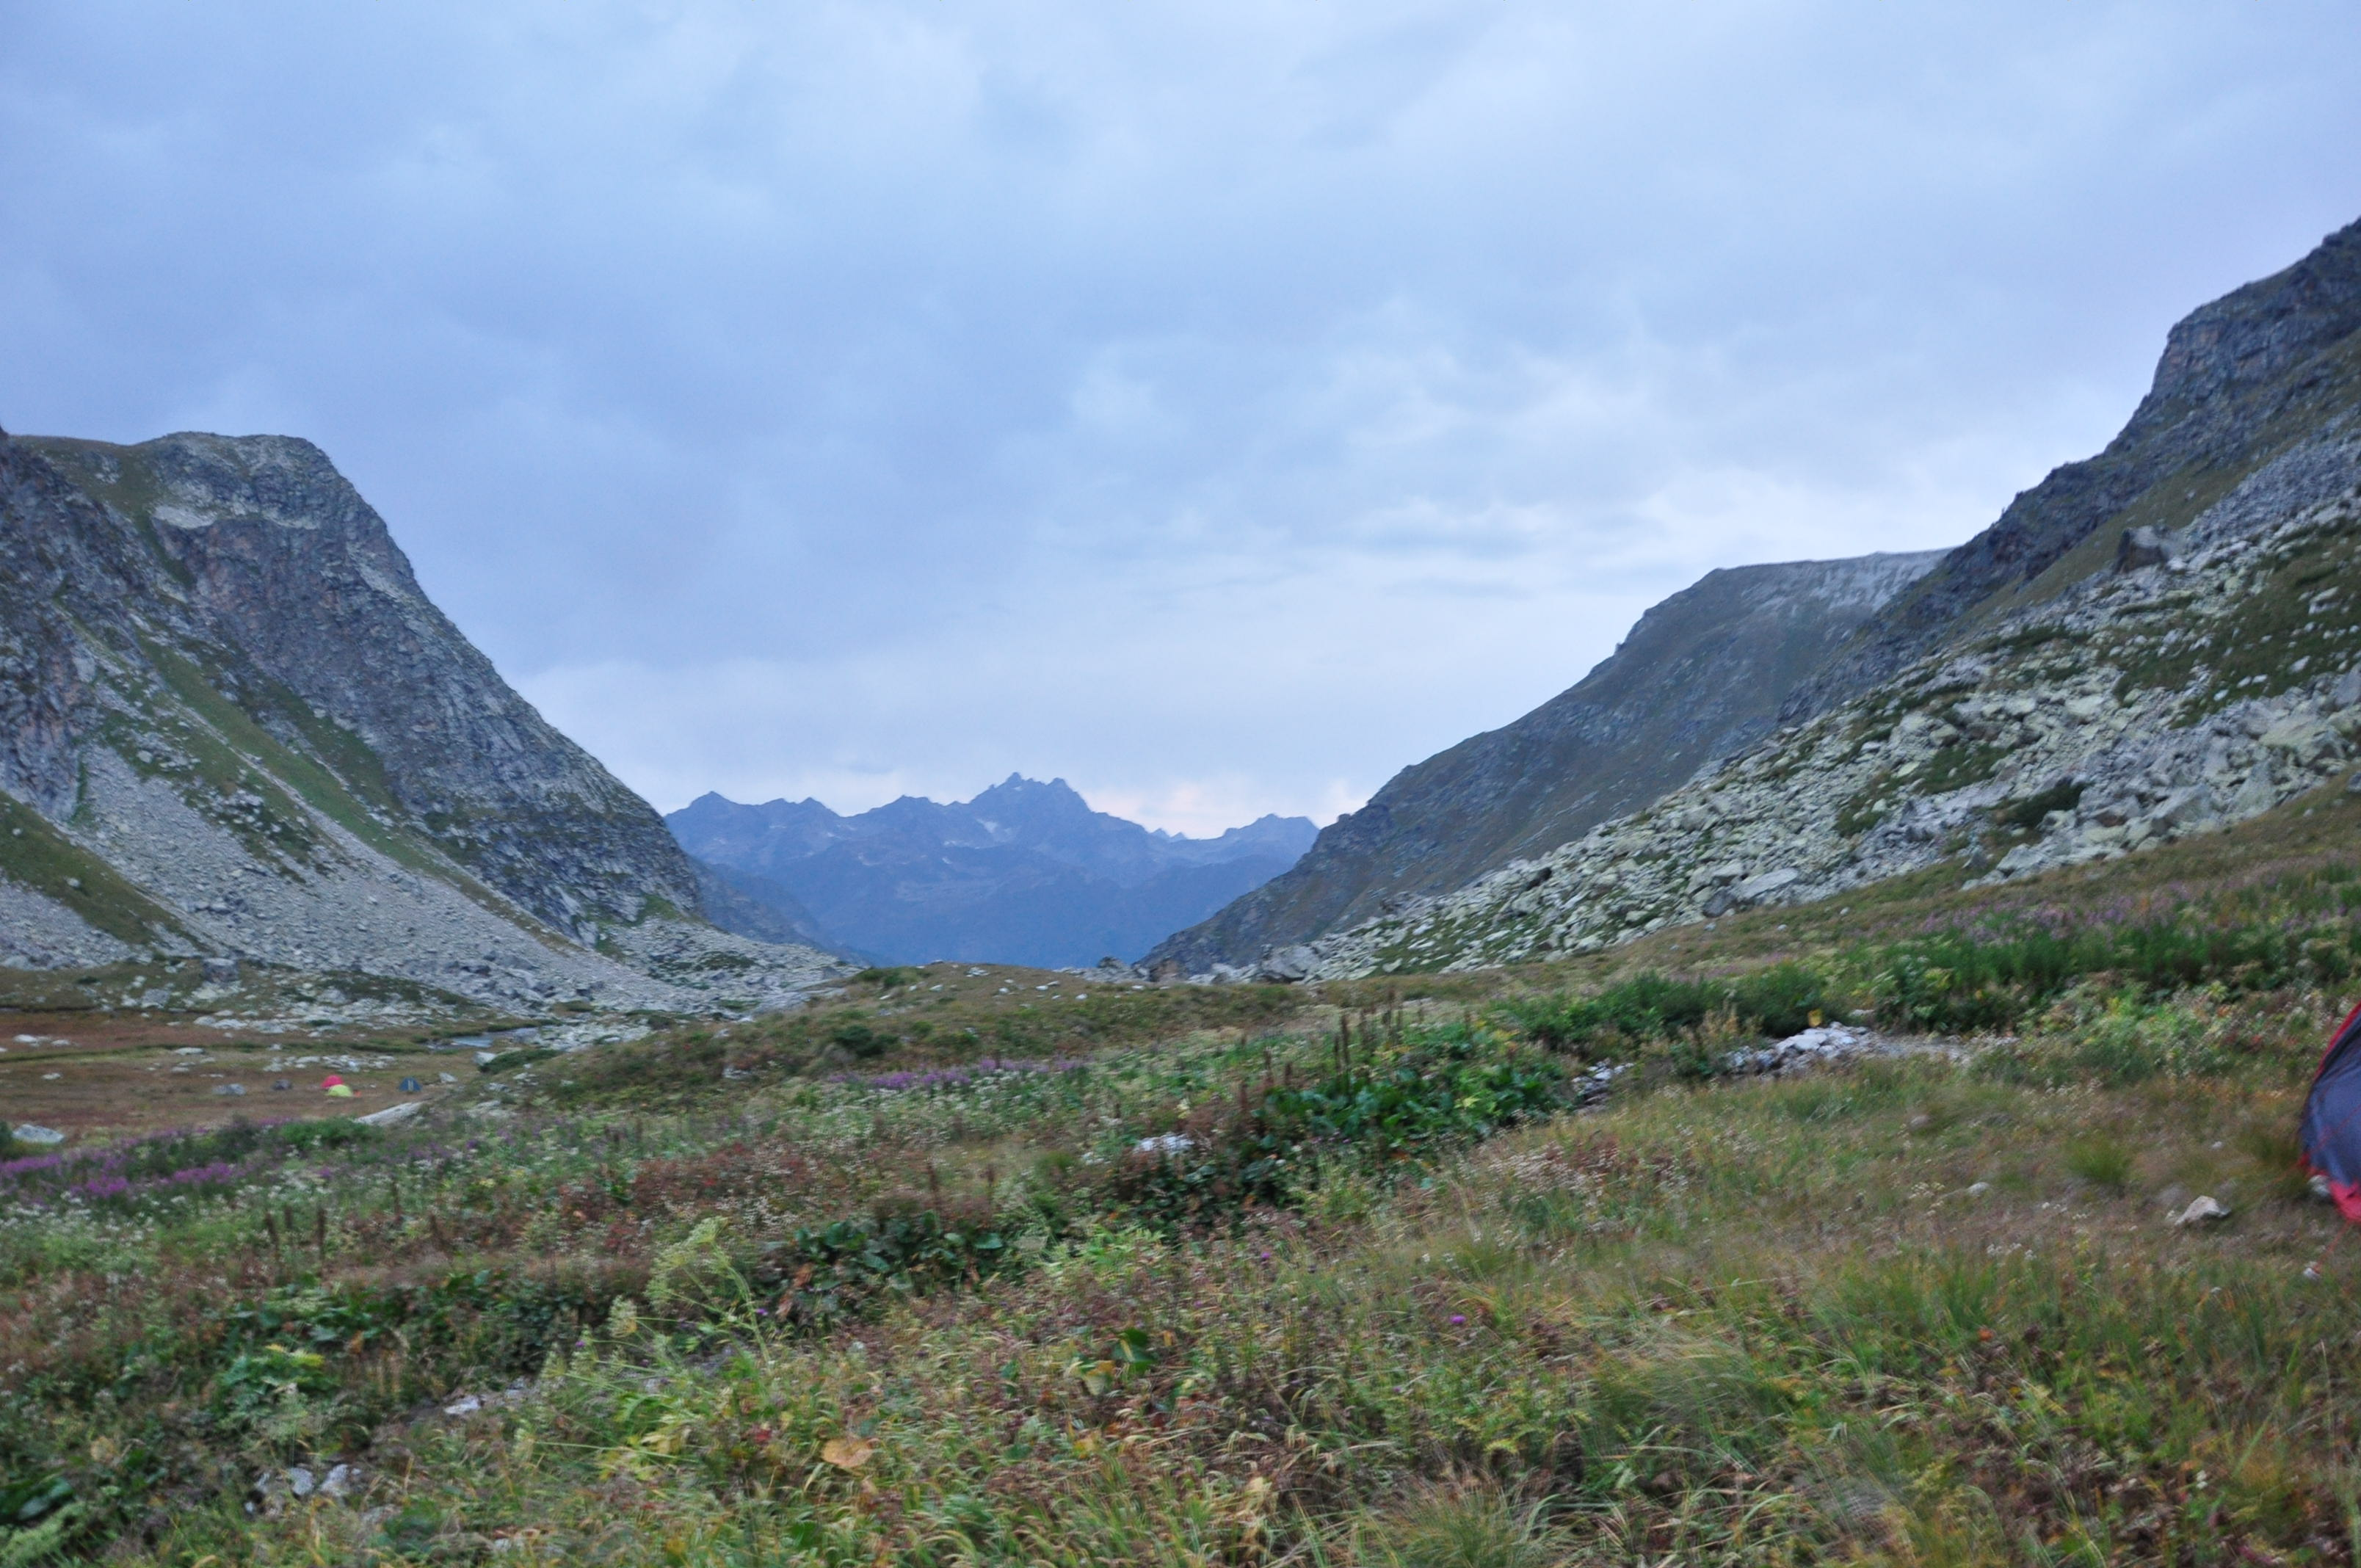
\includegraphics[width=0.7\linewidth]{../pics/DSC_0018}
	\caption{Место ночёвки 22-23.08}
	\label{fig:DSC_0018}
\end{figure}

\clearpage